% !TeX document-id = {52afcdfc-e5de-44c9-a0fc-d554c25c3963}
% !TeX TXS-program:compile = txs:///arara
% arara: lualatex: {shell: no, synctex: yes, interaction: batchmode}
% arara: lualatex: {shell: no, synctex: yes, interaction: batchmode} if found('log', 'undefined references')

\documentclass[a4paper,11pt]{article}
\usepackage[revgoku,breakable]{cp-base}
\graphicspath{{./graphics/}}
%variables
\donnees[%
	classe={1\up{ère} 2M2},matiere={[SPÉ.MATHS]},mois=Octobre,annee=2021,typedoc=CHAP,numdoc=2]

%formatage
\author{Pierquet}
\title{\nomfichier}
\hypersetup{pdfauthor={Pierquet},pdftitle={\nomfichier},allbordercolors=white,pdfborder=0 0 0,pdfstartview=FitH}
%divers
\lhead{\entete{\matiere}}
\chead{\entete{\lycee}}
\rhead{\entete{\classe{} - \mois{} \annee}}
\lfoot{\pied{\matiere}}
\cfoot{\logolycee{}}
\rfoot{\pied{\numeropagetot}}

\begin{document}

\pagestyle{fancy}

\part{CH02 - Suites numériques - Exercices (Correction)}

\smallskip

\exonum{0}

\begin{enumerate}[itemsep=0pt]
	\item On a (formule explicite) $u_0=0^3+3 \times 0 -1 = -1$ et $u_1=1^3+3\times1-1=3$.
	\item On a, de même, $u_{10}=10^3+3\times10-1=\num{1029}$.
	\item \begin{itemize}[leftmargin=*]
		\item On a ${\red u_n} + 1 = {\red n^3+3n-1}+1=n^3+3n$ ;
		\item $u_{\red n+1}=({\red n+1})^3+3({\red n+1})-1=n^3+3n^2+3n+1+3n+3-1=n^3+3n^2+6n$. (qui est différent de $u_n + 1$ !)
	\end{itemize}
\end{enumerate}

\medskip

\exonum{0}

\begin{enumerate}[itemsep=0pt]
	\item On a (formule explicite) $u_0=\dfrac{0-3}{0+2}=-1,5$ et $u_1=\dfrac{1-3}{1+2}=-\dfrac{2}{3}$.
	\item La suite $\suiten$ est définie par une formule explicite.
	\item La fonction $f$ associée à la suite $\suiten$ est $f(x)=\dfrac{x-3}{x+2}$ (on remplace $n$ par $x$ !).
	\item On a $u_{50}=\dfrac{50-3}{50+2}=\dfrac{47}{52}$.
\end{enumerate}

\medskip

\exonum{1}

\begin{enumerate}[itemsep=0pt]
	\item On a (formule de récurrence) :
	\begin{itemize}
		\item $u_1=2u_0-3=2 \times 4 -3 = 5$ ;
		\item $u_2=2u_1-3=2 \times 5 - 3=7$.
	\end{itemize}
	\item La suite $\suiten$ est définie par récurrence.
	\item La fonction $f$ associée à la suite $\suiten$ est $f(x)=2x-3$ (on remplace $u_n$ par $x$ !).
	\item Le module \ccalg{Suites} de la calculatrice donne $u_{15}=\num{32771}$.
	\begin{center}
		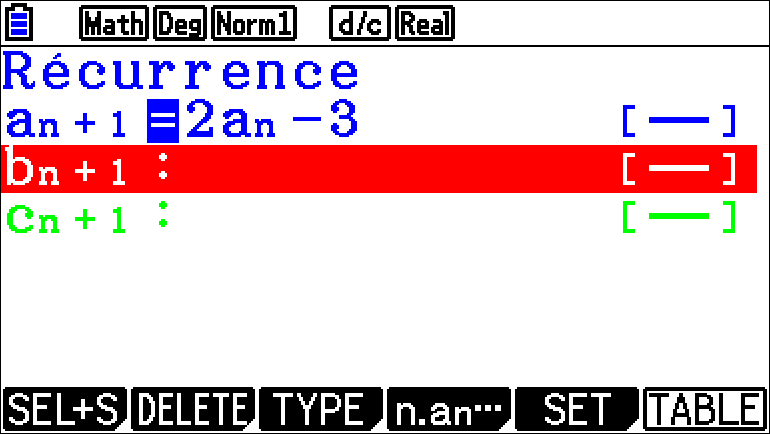
\includegraphics[height=2.5cm]{chap02_exos_corr_3a}~~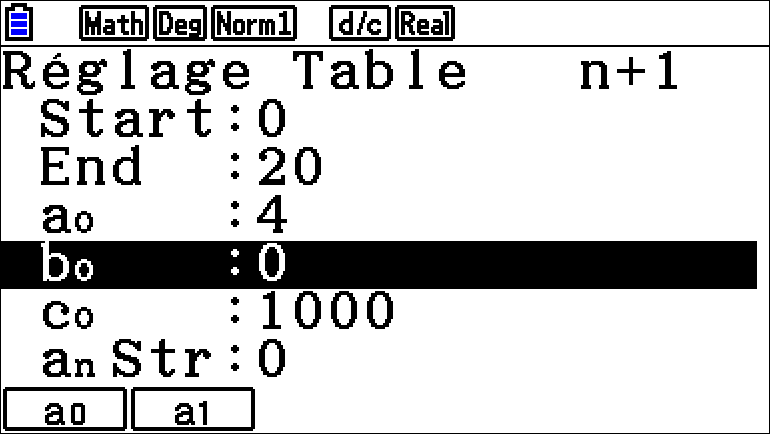
\includegraphics[height=2.5cm]{chap02_exos_corr_3b}~~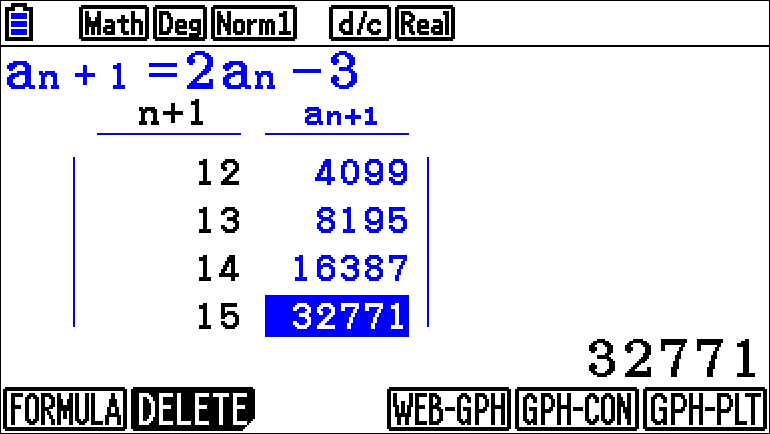
\includegraphics[height=2.5cm]{chap02_exos_corr_3c}
	\end{center}
\end{enumerate}

\medskip

\exonum{1}

\begin{enumerate}[itemsep=0pt]
	\item On a (formule de récurrence) :
	\begin{itemize}
		\item $u_1=\dfrac{u_0+2}{u_0^2+1}=\dfrac{1+2}{1^2+1}=\dfrac{3}{2}=1,5$ ;
		\item $u_2=\dfrac{u_1+2}{u_1^2+1}=\dfrac{1,5+2}{1,5^2+1}=\dfrac{14}{13}$.
	\end{itemize}
	\item La suite $\suiten$ est définie par récurrence.
	\item La fonction $f$ associée à la suite $\suiten$ est $f(x)=\dfrac{x+2}{x^2+1}$ (on remplace $u_n$ par $x$ !).
	\item Le module \ccalg{Suites} de la calculatrice donne $u_{20}\approx 1,2517$ (arrondi à $10^{-4}$).
	\begin{center}
		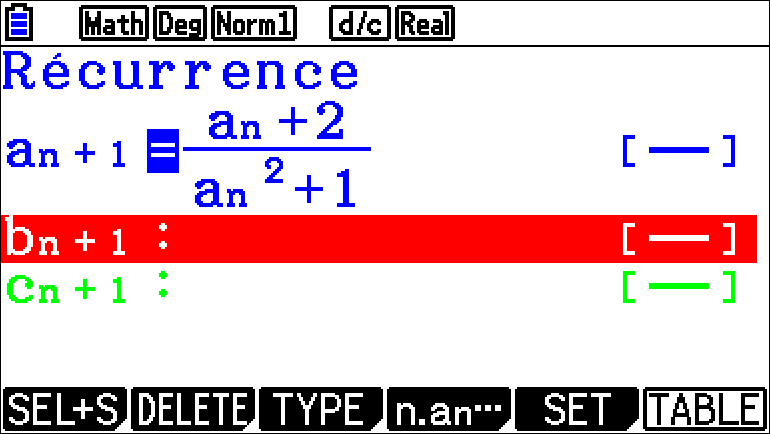
\includegraphics[height=2.5cm]{chap02_exos_corr_4a}~~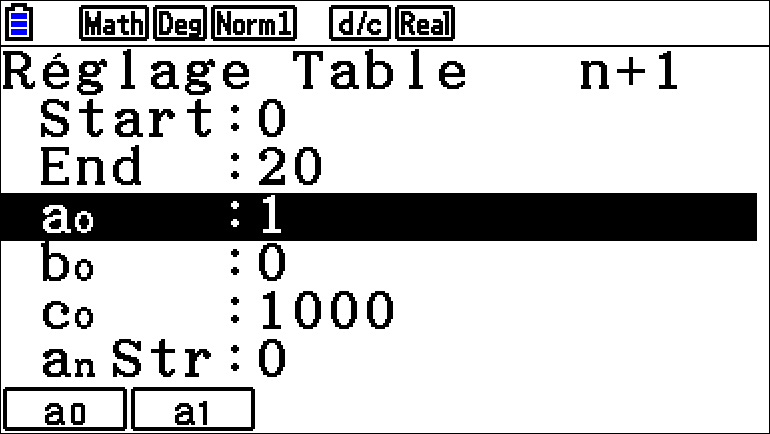
\includegraphics[height=2.5cm]{chap02_exos_corr_4b}~~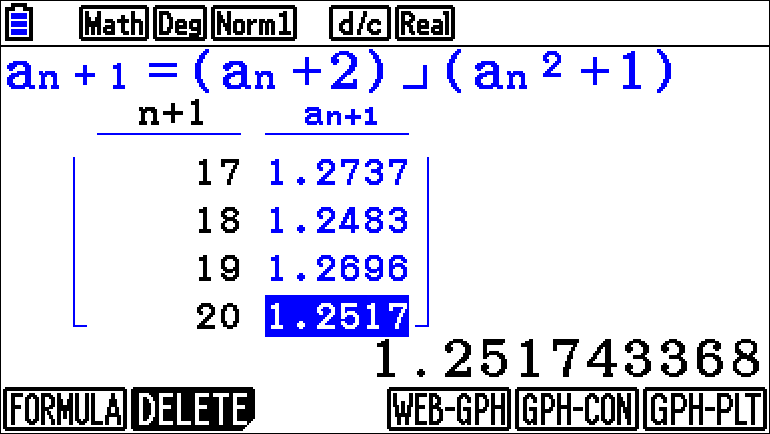
\includegraphics[height=2.5cm]{chap02_exos_corr_4c}
	\end{center}
\end{enumerate}

\medskip

\exonum{1}

\begin{enumerate}[itemsep=0pt]
	\item Il s'agit d'une suite récurrente \og non classique \fg{} pour laquelle il faut respecter la concordance d'indice !
	
	$u_{{\red n}+1}={\red n}-u_{{\red n}}$ :
	\begin{itemize}
		\item $u_1=u_{{\red 0}+1}={\red 0}-u_{\red 0}=0-10=-10$ ;
		\item $u_2=u_{{\red 1}+1}={\red 1}-u_{\red 1}=1-(-10)=11$.
	\end{itemize}
	\item Le module \ccalg{Suites} de la calculatrice donne $u_{18}=19$.
	\begin{center}
		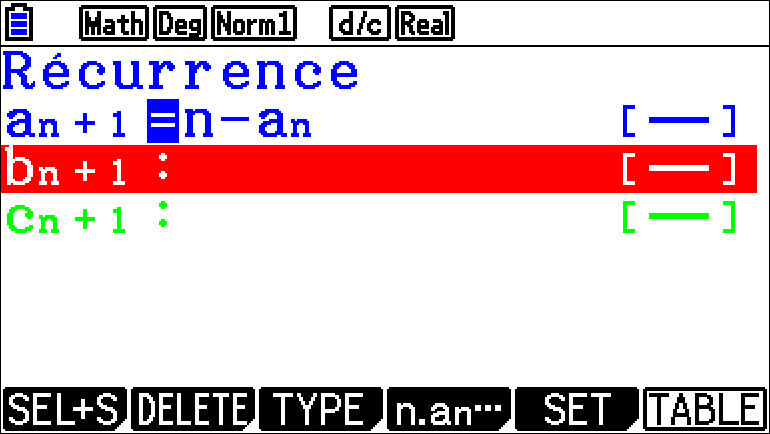
\includegraphics[height=2.5cm]{chap02_exos_corr_5a}~~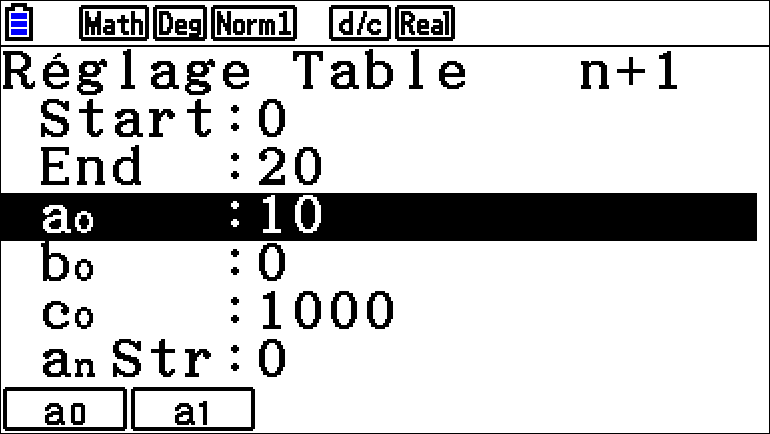
\includegraphics[height=2.5cm]{chap02_exos_corr_5b}~~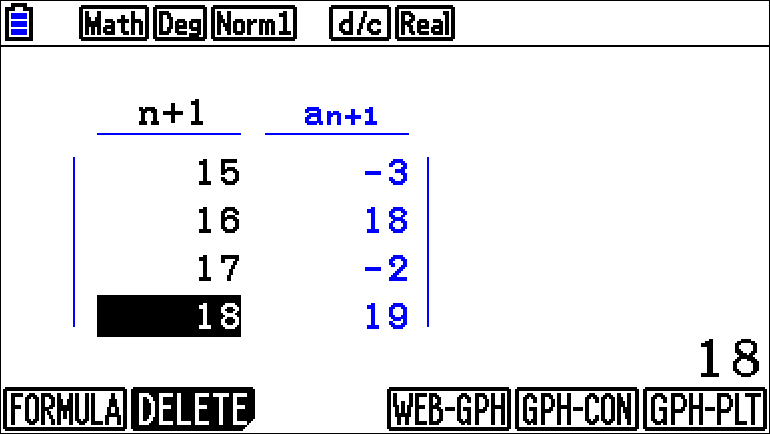
\includegraphics[height=2.5cm]{chap02_exos_corr_5c}
	\end{center}
\end{enumerate}

\medskip

\exonum{3}

\begin{enumerate}[itemsep=0pt]
	\item Il s'agit d'une suite récurrente \og non classique \fg{} pour laquelle il faut respecter la concordance d'indice !
	
	$v_{{\red n}+1}=\dfrac{({\red n}+1)v_{\red n}}{{\red n}(1+v_{\red n})}$ :
	\begin{itemize}
		\item $v_2=v_{{\red 1}+1}=\dfrac{({\red 1}+1)v_{\red 1}}{{\red 1}(1+v_{\red 1})}=\dfrac{2v_1}{1(1+v_1)}=\dfrac{2 \times 4}{1+4}=1,6$ ;
		\item $v_3=v_{{\red 2}+1}=\dfrac{({\red 2}+1)v_{\red 2}}{{\red 2}(1+v_{\red 2})}=\dfrac{3v_2}{2(1+v_2)}=\dfrac{12}{13}$ ;
		\item $v_4=v_{{\red 3}+1}=\dfrac{({\red 3}+1)v_{\red 3}}{{\red 3}(1+v_{\red 3})}=\dfrac{4v_3}{3(1+v_3)}=0,64$.
	\end{itemize}
	\item Le module \ccalg{Suites} de la calculatrice donne $v_{11}=\dfrac{44}{221}\approx 0,199$ (arrondi au millième).
	\begin{center}
		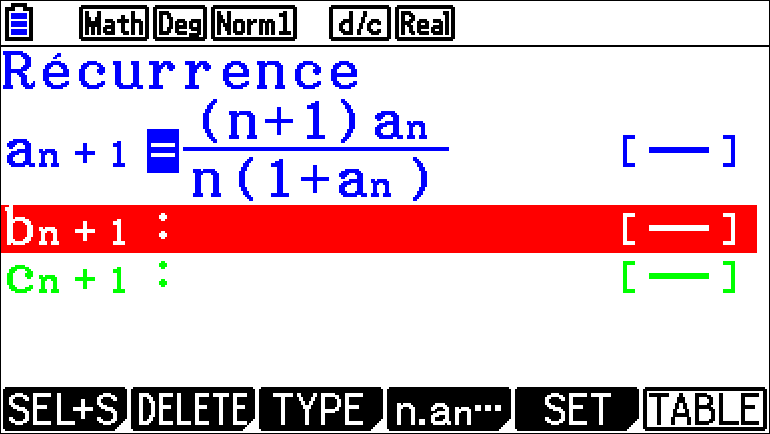
\includegraphics[height=2.5cm]{chap02_exos_corr_6a}~~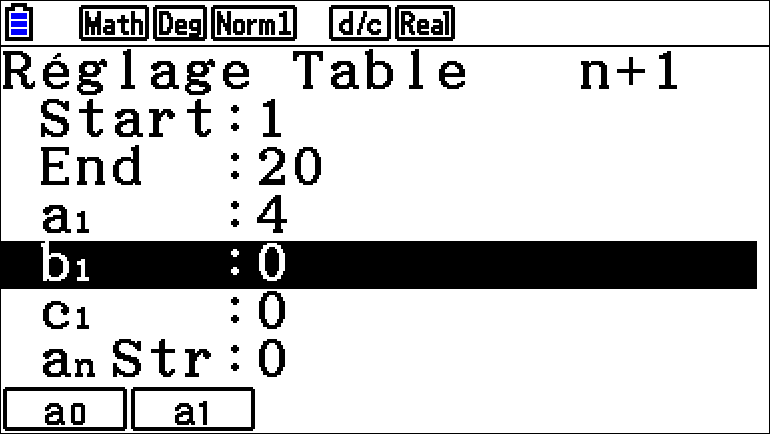
\includegraphics[height=2.5cm]{chap02_exos_corr_6b}~~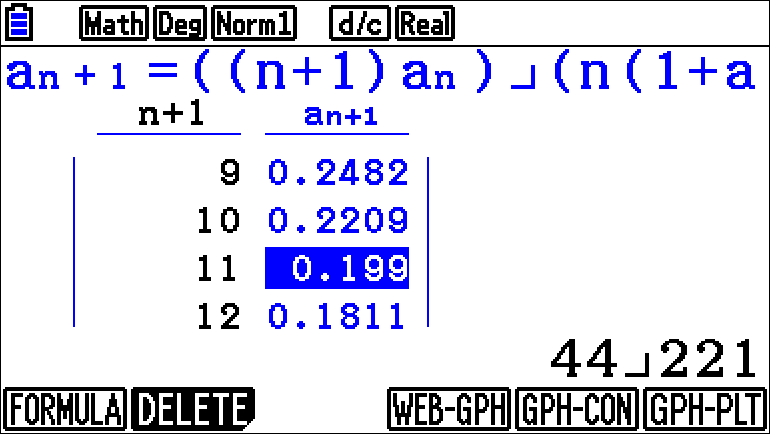
\includegraphics[height=2.5cm]{chap02_exos_corr_6c}
	\end{center}
\end{enumerate}

\medskip

\exonum{2}

\begin{enumerate}[itemsep=0pt]
	\item On a $v_0=\dfrac{(-1)^0}{0+1}=1$ et $v_1=\dfrac{(-1)^1}{1+1}=-0,5$ et $v_2=\dfrac{(-1)^2}{2+1}=\dfrac13$ et $v_3=\dfrac{(-1)^1}{3+1}=-0,25$ et $v_4=\dfrac{(-1)^4}{4+1}=0,2$.
	\item On a :
	\begin{itemize}
		\item $v_{2n}=\dfrac{(-1)^{2n}}{(2n)+1}=\dfrac{1}{2n+1} > 0$ ;
		\item $v_{2n+1}=\dfrac{(-1)^{2n+1}}{(2n+1)+1}=\dfrac{-1}{2n+2} < 0$.
	\end{itemize}
\end{enumerate}

\pagebreak

\exonum{1}

\begin{enumerate}[itemsep=0pt]
	\item On a (formule explicite) $w_0=\dfrac{2}{5^0}=2$ et  $w_1=\dfrac{2}{5^1}=0,4$ et $w_2=\dfrac{2}{5^2}=0,08$ et $w_3=\dfrac{2}{5^3}=0,016$.
	\item On a $\dfrac{w_{n+1}}{w_n} = \dfrac{\tfrac{2}{5^{n+1}}}{\tfrac{2}{5^{n}}}=\dfrac{2}{5^{n+1}} \times \dfrac{5^n}{2}=\dfrac{5^n}{5^{n+1}}=\dfrac{5^n}{5^n \times 5}=\dfrac{1}{5}$ qui est bien indépendant de $n$ !
\end{enumerate}

\medskip

\exonum{3}

\begin{enumerate}[itemsep=0pt]
	\item On a (formule explicite) $u_1=1+\dfrac11=2$ et $u_2=1+\dfrac12=1,5$ et $u_3=1+\dfrac13=\dfrac43$ puis $u_{15}=1+\dfrac{1}{15}=\dfrac{16}{15}$.
	\item On représente le nuage de points :
	\begin{center}
		\tunits{1}{1}
		\tdefgrille{0}{10}{1}{1}{0}{2.5}{0.5}{0.5}
		\begin{tikzpicture}[x=\xunit cm,y=\yunit cm]
			\tgrilles[line width=0.4pt,lightgray]
			\axestikz* \axextikz{0,1,...,9} \axeytikz{0,0.5,1,1.5,2}
			\foreach \n in {1,2,...,10}
				\filldraw[red] (\n,{1+1/\n}) circle[radius=2.5pt] ;
		\end{tikzpicture}
	\end{center}
	\item On peut conjecturer que $\suiten$ est monotone décroissante et convergente vers $\ell=1$.
	\item 
	\begin{enumerate}[itemsep=0pt]
		\item On a $u_{n+1}-u_n = 1+\dfrac{1}{n+1} - \left( 1+\dfrac{1}{n} \right) = \dfrac{1}{n+1} - \dfrac{1}{n} = \dfrac{n}{n(n+1)} - \dfrac{n+1}{n(n+1)} = \dfrac{n-(n+1)}{n(n+1)} = \dfrac{-1}{n(n+1)}$.
		\item par quotient, on a $u_{n+1}-u_n < 0$ (pour tout $n$ non nul), ce qui justifie que $\suiten$ est monotone décroissante.
	\end{enumerate}
	\item Sachant que $\dfrac{1}{n} >0$, on en déduit que $u_n >1$ pour tout entier $n$ non nul.
\end{enumerate}

\medskip

\exonum{3}

\begin{enumerate}[itemsep=0pt]
	\item On a (formule de récurrence) :
	\begin{itemize}
		\item $v_1=-0,25v_0^2+v_0=-0,25 \times 2^2+2 = 1$ ;
		\item $v_2=-0,25v_1^2+v_1=-0,25 \times 1^2+1 = 0,75$ ;
		\item $v_3=-0,25v_2^2+v_2=-0,25 \times 0,75^2+0,75 = \dfrac{39}{64} = \num{0,609375}$.
	\end{itemize}
	\item 
	\begin{enumerate}[itemsep=0pt]
		\item La fonction $f$ telle que $v_{n+1} = f(v_n)$ est $f(x)=-0,25x^2+x$ (on remplace $u_n$ par $x$ !).
		\item À l'aide de la technique de la \og toile \fg{} :
		\begin{center}
			\tunits{4}{3}
			\tdefgrille{0}{2.5}{0.25}{0.25}{0}{1.25}{0.25}{0.25}
			\begin{tikzpicture}[x=\xunit cm,y=\yunit cm]
				\tgrilles[line width=0.4pt,lightgray] ;
				\axestikz \axextikz{0,1,2} ;
				\foreach \y in {0,0.25,0.5,0.75,1.0}
					\draw[line width=1.25pt] (4pt,\y) -- (-4pt,\y) node[left] {\num{\y}} ;
				\clip (\xmin,\ymin) rectangle (\xmax,\ymax) ;
				\draw[line width=1.25pt,red](0,0) -- (1.25,1.25) ;
				\draw[line width=1.25pt,blue,domain=0:2.5,samples=200] plot (\x,{-0.25*\x*\x+\x}) ;
				\draw (1.25,1.25) node[below right] {\large \red $\Delta$ : $y=x$} ;
				\draw (2,1) node[above right] {\large \blue $\mathscr{C}_f$} ;
				\draw[ForestGreen,ultra thick] (2,0)--(2,1)--(1,1)--(1,0.75)--(0.75,0.75)--(0.75,0.609375)--(0.609375,0.609375)--(0.609375,0.51654)--(0.51654,0.51654) ;
			\end{tikzpicture}
		\end{center}
		\item On peut conjecturer que $\suiten[v]$ est monotone décroissante et convergente vers $\ell=0$.
	\end{enumerate}
	\item On a $v_{n+1}-v_n=-0,25v_n^2+v_n-v_n=-0,25v_n^2 < 0$ pour tout entier naturel $n$, donc on en déduit que $\suiten[v]$ est décroissante.
\end{enumerate}

\end{document}